\documentclass[10pt]{article}
\usepackage[margin=18mm]{geometry}
\usepackage{graphicx,booktabs,hyperref}
\usepackage[strings]{underscore}
\setlength{\parindent}{0pt}\setlength{\parskip}{5pt}
\begin{document}
\section*{Exact support diagnosis of the n=7 smoke}

Post-outcome correctness diagnosis, 2026-10-25, protocol amendment 5.
The failed frozen session is ECBS1h1572078f47bd; it exhausted all ten
records including both rho controls. This diagnosis changes none of them.

The K0 model has field degree 7, group order 116, prime subgroup r=29 and
cofactor 4: icv1-f2m7-t13-616700dd. Its geometric dimension-2 base, seed 17,
has four signed points. Exhaustive enumeration of all 64 ordered triples
including repeated points finds zero sums in the prime subgroup. Hence
none of these three-summand arms can produce a prime-subgroup relation on
this exact base; this is a finite support fact, not a failure of F4.
Exact identity: \path{ICV1:f2m-7-e1a6f45a:13:116:0x1:-7:unk:r:616700ddc6fe};
subgroup generator (0x26,0x5).

\begin{center}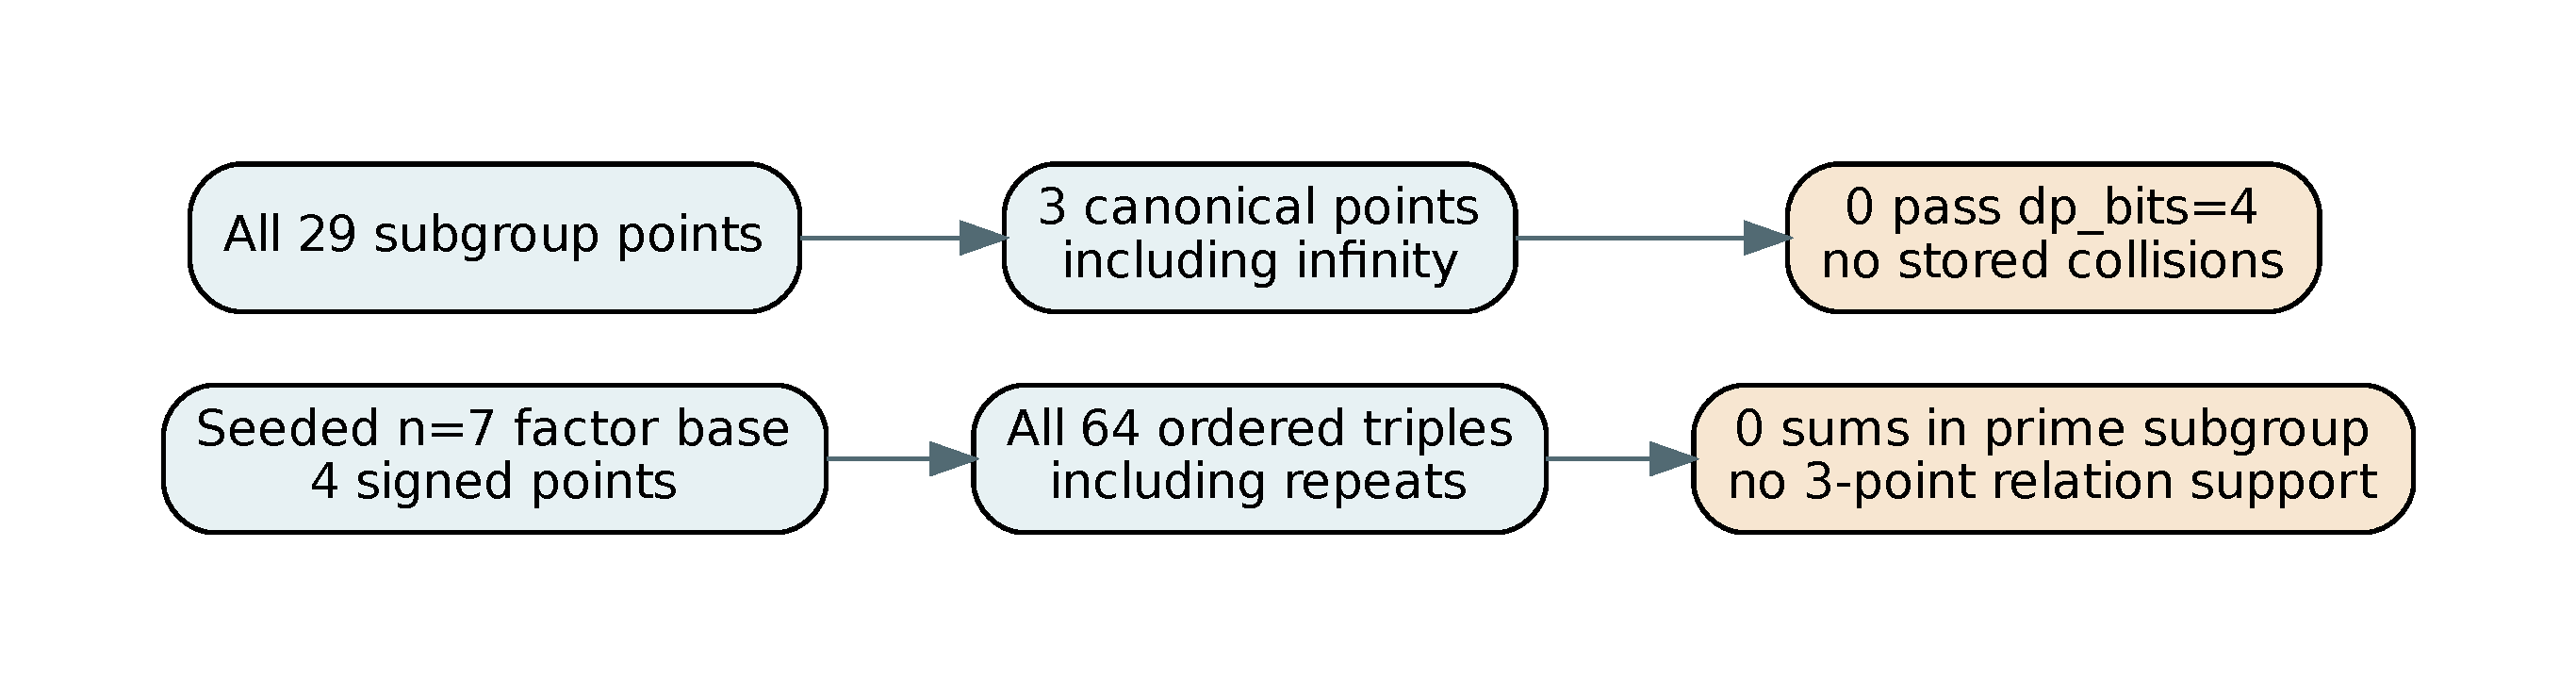
\includegraphics[width=.98\linewidth]{finite-support.pdf}\end{center}

Enumerating every scalar 0--28 gives three signed-Frobenius canonical
representatives including infinity. The low hexadecimal digits of their
source-pinned distinguished hashes are 2,3,7. None passes the frozen
four-bit distinguished predicate. No canonical point can enter its rho
collision table under this configuration. This explains the independent
reference failure without treating it as zero rho cost.

Native source: examples/ic_structured_small_audit.rs. Complete coordinates,
r-multiples, canonical points and hashes, plus source SHA-256 pins, are in
pipeline-receipts/structured-n7-support.json. It reuses actual base construction
and public strong-rho canonicalization, and implements the literal private
hash from the pinned source. Re-run the native example to check the finite
enumeration. No timings are reported; the diagram shows separate failure paths
because the two counts have different domains.

This does not establish failure on any other basis or field, retune the
original reference, qualify a performance comparison, or prove a generic
obstruction. A separately frozen viable tiny fixture is needed for that role.

\end{document}
